``A continuación, se presentan distintas cuestiones relacionadas con las sensaciones y el comportamiento que tiene ante las incorporaciones a las autovías. Responda rápido, considerando que no hay respuestas correctas. Simplemente, responda con la respuesta que mejor caracterice cómo se siente usted ante una incorporación en autovía. Los datos recogidos son anónimos.''



1. Cuando me incorporo a una autovía me siento nervioso
\vspace{-10pt}
\begin{table}[htbp]
\centering
\begin{tabular}{|c|c|c|c|c|}
\hline
Nunca o casi nunca & Pocas veces & A veces & Muchas veces & Siempre o casi siempre \\ \hline
\end{tabular}
\end{table}


2. Si voy de copiloto y el coche se acerca a una incorporación me comporto como si fuera yo el conductor (por ejemplo, mirando el tráfico y los espejos) 
\vspace{-10pt}
\begin{table}[h]
\centering
\begin{tabular}{|c|c|c|c|c|}
\hline
Nunca o casi nunca & Pocas veces & A veces & Muchas veces & Siempre o casi siempre \\ \hline
\end{tabular}
\end{table}


3. Si voy a incorporarme una autovía y los ocupantes del vehículo me están hablando me siento tenso
\vspace{-10pt}
\begin{table}[h]
\centering
\begin{tabular}{|c|c|c|c|c|}
\hline
Nunca o casi nunca & Pocas veces & A veces & Muchas veces & Siempre o casi siempre \\ \hline
\end{tabular}
\end{table}

4. Indique de 1 a 5 el nivel de estrés, siendo 1 poco o muy poco y 5 mucho, que le podría producir una incorporación como las siguientes 
\newpage
\vspace{-10pt}
\begin{table}[]
\centering
\begin{tabular}{|r|l|l|l|l|l|}
\hline
\textit{}                             & \textbf{1} & \textbf{2} & \textbf{3} & \textbf{4} & \textbf{5} \\ \hline
Con señal de STOP                     & \textit{}  & \textit{}  & \textit{}  & \textit{}  & \textit{}  \\ \hline
Con señal de ceda el paso             &            &            &            &            &            \\ \hline
Con carril de aceleración largo       &            &            &            &            &            \\ \hline
Con carril de aceleración corto       &            &            &            &            &            \\ \hline
Con una curva cerrada                 &            &            &            &            &            \\ \hline
Perteneciente a un nudo de carreteras &            &            &            &            &            \\ \hline
\end{tabular}
\end{table}

5. Me siento nervioso si no me facilitan la incorporación a una autovía y pienso que voy a tener que frenar 
\vspace{-10pt}
\begin{table}[h]
\centering
\begin{tabular}{|c|c|c|c|c|}
\hline
Nunca o casi nunca & Pocas veces & A veces & Muchas veces & Siempre o casi siempre \\ \hline
\end{tabular}
\end{table}

6. Me siento nervioso si llego al final del carril muy lento 
\vspace{-10pt}
\begin{table}[h]
\centering
\begin{tabular}{|c|c|c|c|c|}
\hline
Nunca o casi nunca & Pocas veces & A veces & Muchas veces & Siempre o casi siempre \\ \hline
\end{tabular}
\end{table}

7. Me siento tenso si en condiciones de baja visibilidad o luminosidad (niebla, lluvia, de noche…) tengo que realizar una incorporación
% \vspace{-10pt}
\begin{table}[H]
\centering
\begin{tabular}{|c|c|c|c|c|}
\hline
Nunca o casi nunca & Pocas veces & A veces & Muchas veces & Siempre o casi siempre \\ \hline
\end{tabular}
\end{table}

8. Sabiendo que no suele haber tráfico en la vía donde me voy a incorporar, me siento tranquilo y acelero
\vspace{-10pt}
\begin{table}[H]
\centering
\begin{tabular}{|c|c|c|c|c|}
\hline
Nunca o casi nunca & Pocas veces & A veces & Muchas veces & Siempre o casi siempre \\ \hline
\end{tabular}
\end{table}

9. Si me encuentro un camión o autobús en el carril donde quiero incorporarme, me resulta estresante
\vspace{-10pt}
\begin{table}[H]
\centering
\begin{tabular}{|c|c|c|c|c|}
\hline
Nunca o casi nunca & Pocas veces & A veces & Muchas veces & Siempre o casi siempre \\ \hline
\end{tabular}
\end{table}

10. Disfruto incorporándome a una autovía
\vspace{-10pt}
\begin{table}[H]
\centering
\begin{tabular}{|c|c|c|c|c|}
\hline
Nunca o casi nunca & Pocas veces & A veces & Muchas veces & Siempre o casi siempre \\ \hline
\end{tabular}
\end{table}

11. Me gusta realizar maniobras bruscas cuando me incorporo
\vspace{-10pt}
\begin{table}[H]
\centering
\begin{tabular}{|c|c|c|c|c|}
\hline
Nunca o casi nunca & Pocas veces & A veces & Muchas veces & Siempre o casi siempre \\ \hline
\end{tabular}
\end{table}

12. Espero hasta el final para frenar cuando realizo una incorporación
\vspace{-10pt}
\begin{table}[h]
\centering
\begin{tabular}{|c|c|c|c|c|}
\hline
Nunca o casi nunca & Pocas veces & A veces & Muchas veces & Siempre o casi siempre \\ \hline
\end{tabular}
\end{table}

13. Pienso que si vas con suficiente velocidad los demás conductores te facilitan el paso en una incorporación
\vspace{-10pt}
\begin{table}[h]
\centering
\begin{tabular}{|c|c|c|c|c|}
\hline
Nunca o casi nunca & Pocas veces & A veces & Muchas veces & Siempre o casi siempre \\ \hline
\end{tabular}
\end{table}

14. Cuando las condiciones me lo permiten suelo facilitar la incorporación de otros vehículos a la vía por la que circulo
\vspace{-10pt}
\begin{table}[h]
\centering
\begin{tabular}{|c|c|c|c|c|}
\hline
Nunca o casi nunca & Pocas veces & A veces & Muchas veces & Siempre o casi siempre \\ \hline
\end{tabular}
\end{table}

15. Indica el lugar del carril de aceleración en el que suele parar cuando no puede incorporarse
\vspace{-10pt}
\begin{figure}[H]
    \centering
    \begin{subfigure}[b]{0.4\linewidth}
        \centering
        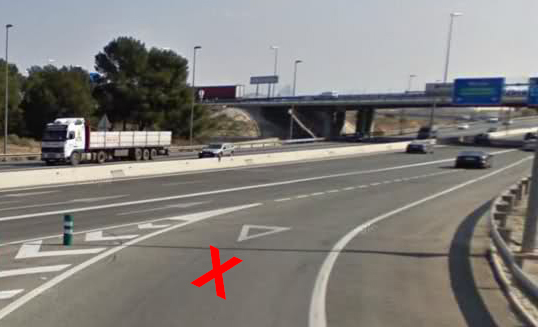
\includegraphics[width=6cm]{figures/A1.jpg}
        \caption{}
    \end{subfigure}
    \hspace{0.5cm}
    \begin{subfigure}[b]{0.4\linewidth}
        \centering
        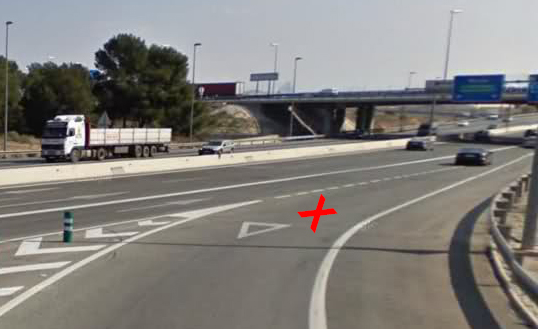
\includegraphics[width=6cm]{figures/A2.jpg}
        \caption{}
    \end{subfigure}
    \begin{subfigure}[b]{0.45\textwidth}
        \centering
        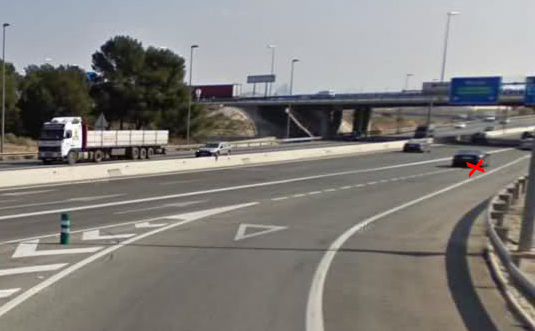
\includegraphics[width=\textwidth]{figures/A3.jpg}
        \caption{}
  \end{subfigure}
\end{figure}

16. Si llevo pasajeros en mi vehículo suelo ser menos arriesgado en las incorporaciones
\vspace{-10pt}
\begin{table}[H]
\centering
\begin{tabular}{|c|c|c|c|c|}
\hline
Nunca o casi nunca & Pocas veces & A veces & Muchas veces & Siempre o casi siempre \\ \hline
\end{tabular}
\end{table}

17. Soy más arriesgado si al incorporarme advierto que tengo vehículos detrás de mí con intención de incorporarse
\vspace{-10pt}
\begin{table}[h]
\centering
\begin{tabular}{|c|c|c|c|c|}
\hline
Nunca o casi nunca & Pocas veces & A veces & Muchas veces & Siempre o casi siempre \\ \hline
\end{tabular}
\end{table}

18. Si un vehículo que va detrás de mí se incorpora primero, de inmediato realizo la maniobra para colocarme por delante de él 
\begin{figure}[h]
    \centering
    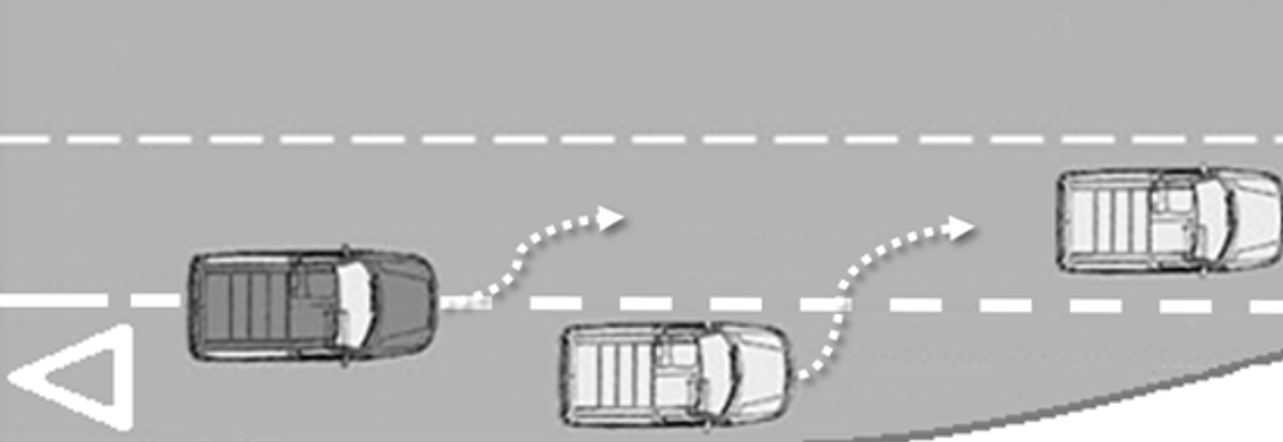
\includegraphics[width=14cm]
    {figures/A4.png}
\end{figure}
   
\vspace{-10pt}
\begin{table}[h]
\centering
\begin{tabular}{|c|c|c|c|c|}
\hline
Nunca o casi nunca & Pocas veces & A veces & Muchas veces & Siempre o casi siempre \\ \hline
\end{tabular}
\end{table}

19. La estrategia que empleo generalmente para incorporarme si hay vehículos en la vía principal es: 
   \begin{itemize}
        \item Acelerar más que ellos y colocarme delante
        \item Reducir la velocidad y dejarlos pasar
        \item Adecuar la velocidad de mi vehículo apurando el espacio entre todos
        \item Otra
   \end{itemize}
\vspace{10pt}

20. Si estas en una vía principal, para facilitar la incorporación: 
   \begin{itemize}
        \item Me cambio de carril
        \item Acelero
        \item Reduzco la velocidad
        \item No suelo facilitar la incorporación
   \end{itemize}
\vspace{-10pt}

\newpage
21. Si un vehículo que va detrás de mí se incorpora primero, de inmediato realizo la maniobra para colocarme por delante de él 
\begin{figure}[h]
    \centering
    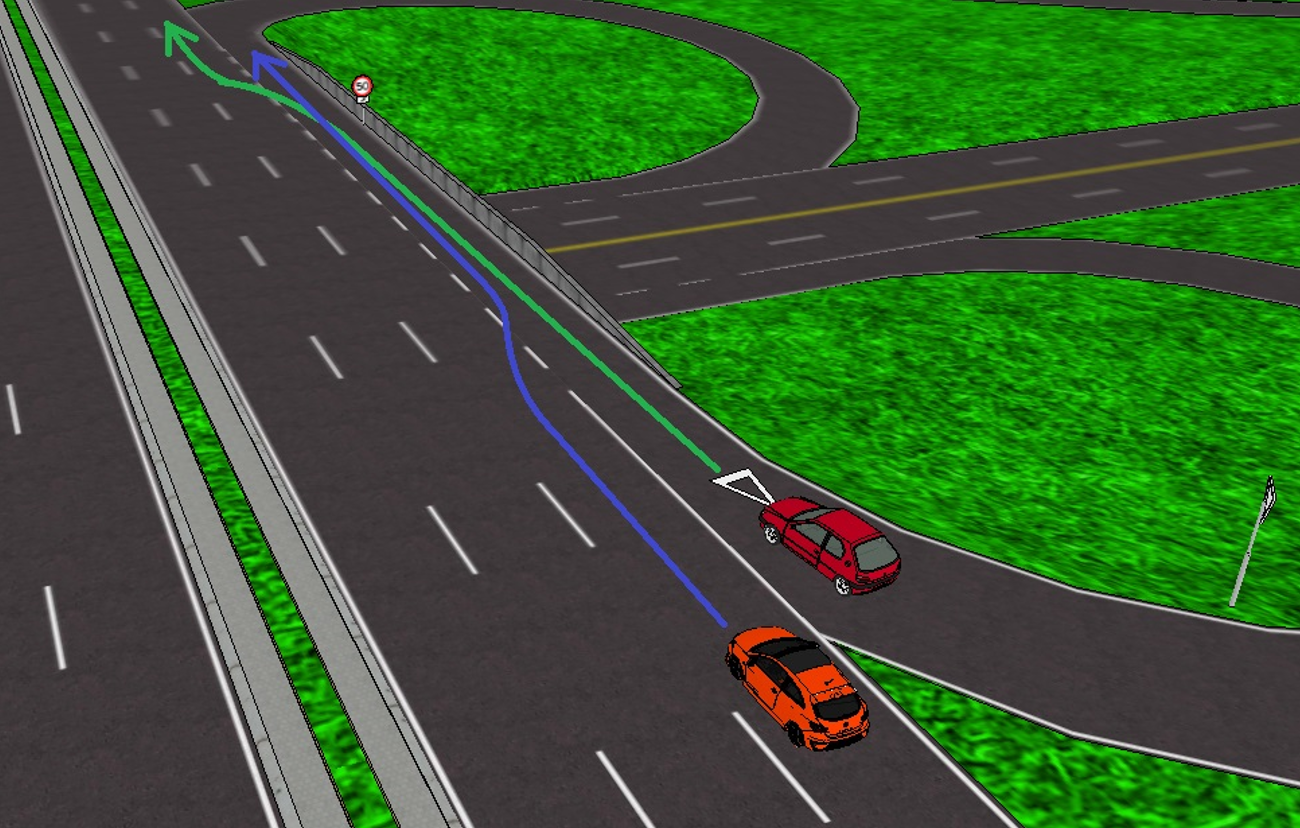
\includegraphics[width=14cm]
    {figures/A5.png}
\end{figure}
\vspace{-10pt}
\begin{table}[h]
\centering
\begin{tabular}{|c|c|c|c|c|}
\hline
Nunca o casi nunca & Pocas veces & A veces & Muchas veces & Siempre o casi siempre \\ \hline
\end{tabular}
\end{table}

22. Si estoy accediendo a una autovía por un carril de incorporación y un vehículo de la vía principal me da las luces largas, creo que:
   \begin{itemize}
        \item Recrimina que no me haya incorporado
        \item Quiere que acelere para incorporarme
        \item Advierte de un peligro
        \item Quiere que frene para dejarle pasar
        \item Otra
   \end{itemize}
\vspace{10pt}

23. Utilizo el claxon en la autovía
\vspace{-10pt}
\begin{table}[h]
\centering
\begin{tabular}{|c|c|c|c|c|}
\hline
Nunca o casi nunca & Pocas veces & A veces & Muchas veces & Siempre o casi siempre \\ \hline
\end{tabular}
\end{table}

24. Utilizo los intermitentes para incorporarme a una autovía
\vspace{-10pt}
\begin{table}[H]
\centering
\begin{tabular}{|c|c|c|c|c|}
\hline
Nunca o casi nunca & Pocas veces & A veces & Muchas veces & Siempre o casi siempre \\ \hline
\end{tabular}
\end{table}

25. Si en el carril de aceleración hay muchos vehículos por delante de mí, rebaso la línea continua en cuanto veo hueco para incorporarme
\vspace{-10pt}
\begin{table}[h]
\centering
\begin{tabular}{|c|c|c|c|c|}
\hline
Nunca o casi nunca & Pocas veces & A veces & Muchas veces & Siempre o casi siempre \\ \hline
\end{tabular}
\end{table}

26. Señale las tres opciones en las que se fija con mayor frecuencia durante una incorporación
   \begin{itemize}
        \item Los vehículos dentro de la vía
        \item El vehículo que tengo detrás
        \item El vehículo que tengo delante
        \item Línea discontinua para entrar
        \item La longitud del carril de aceleración
        \item Señalización de la incorporación
        \item Otra
   \end{itemize}
   \vspace{10pt}
   
27. Durante una incorporación me gusta llevar marchas cortas
\vspace{-10pt}
\begin{table}[h]
\centering
\begin{tabular}{|c|c|c|c|c|}
\hline
Nunca o casi nunca & Pocas veces & A veces & Muchas veces & Siempre o casi siempre \\ \hline
\end{tabular}
\end{table}

28. Cuando el carril de incorporación es corto paro al principio si no tengo clara la salida
\vspace{-10pt}
\begin{table}[h]
\centering
\begin{tabular}{|c|c|c|c|c|}
\hline
Nunca o casi nunca & Pocas veces & A veces & Muchas veces & Siempre o casi siempre \\ \hline
\end{tabular}
\end{table}

29. Tipo de vehículo de uso habitual
   \begin{itemize}
        \item Motocicleta
        \item Turismo
        \item Todoterreno, 4x4, SUV, monovolumen
        \item Furgoneta pequeña
        \item Furgón o furgoneta grande (más de 3,5 toneladas)
        \item Autocar
        \item Camión
        \item Otra
   \end{itemize}
   \vspace{10pt}
   
30. Años con el permiso de conducir
   \vspace{10pt}
   
31. ¿Qué distancia suele recorrer al año en carretera considerando todo tipo de vías? 
   \begin{itemize}
        \item < 5000 km
        \item 5000 - 10000 km
        \item 10000 - 20000 km
        \item >20000 km
        \item Otro
   \end{itemize}
\vspace{10pt}
   
32. Sexo
   \begin{itemize}
        \item Hombre
        \item Mujer
   \end{itemize}
\vspace{10pt}
   
33. Edad
   \vspace{10pt}

